\subsection{Election November 3, 1992: *Clinton vs Bush}
\begin{frame}[t]{Election November 3, 1992: *Bill Clinton}
\small

\begin{columns}[T, onlytextwidth]
\column{0.48\textwidth}
\vspace{-1em}
{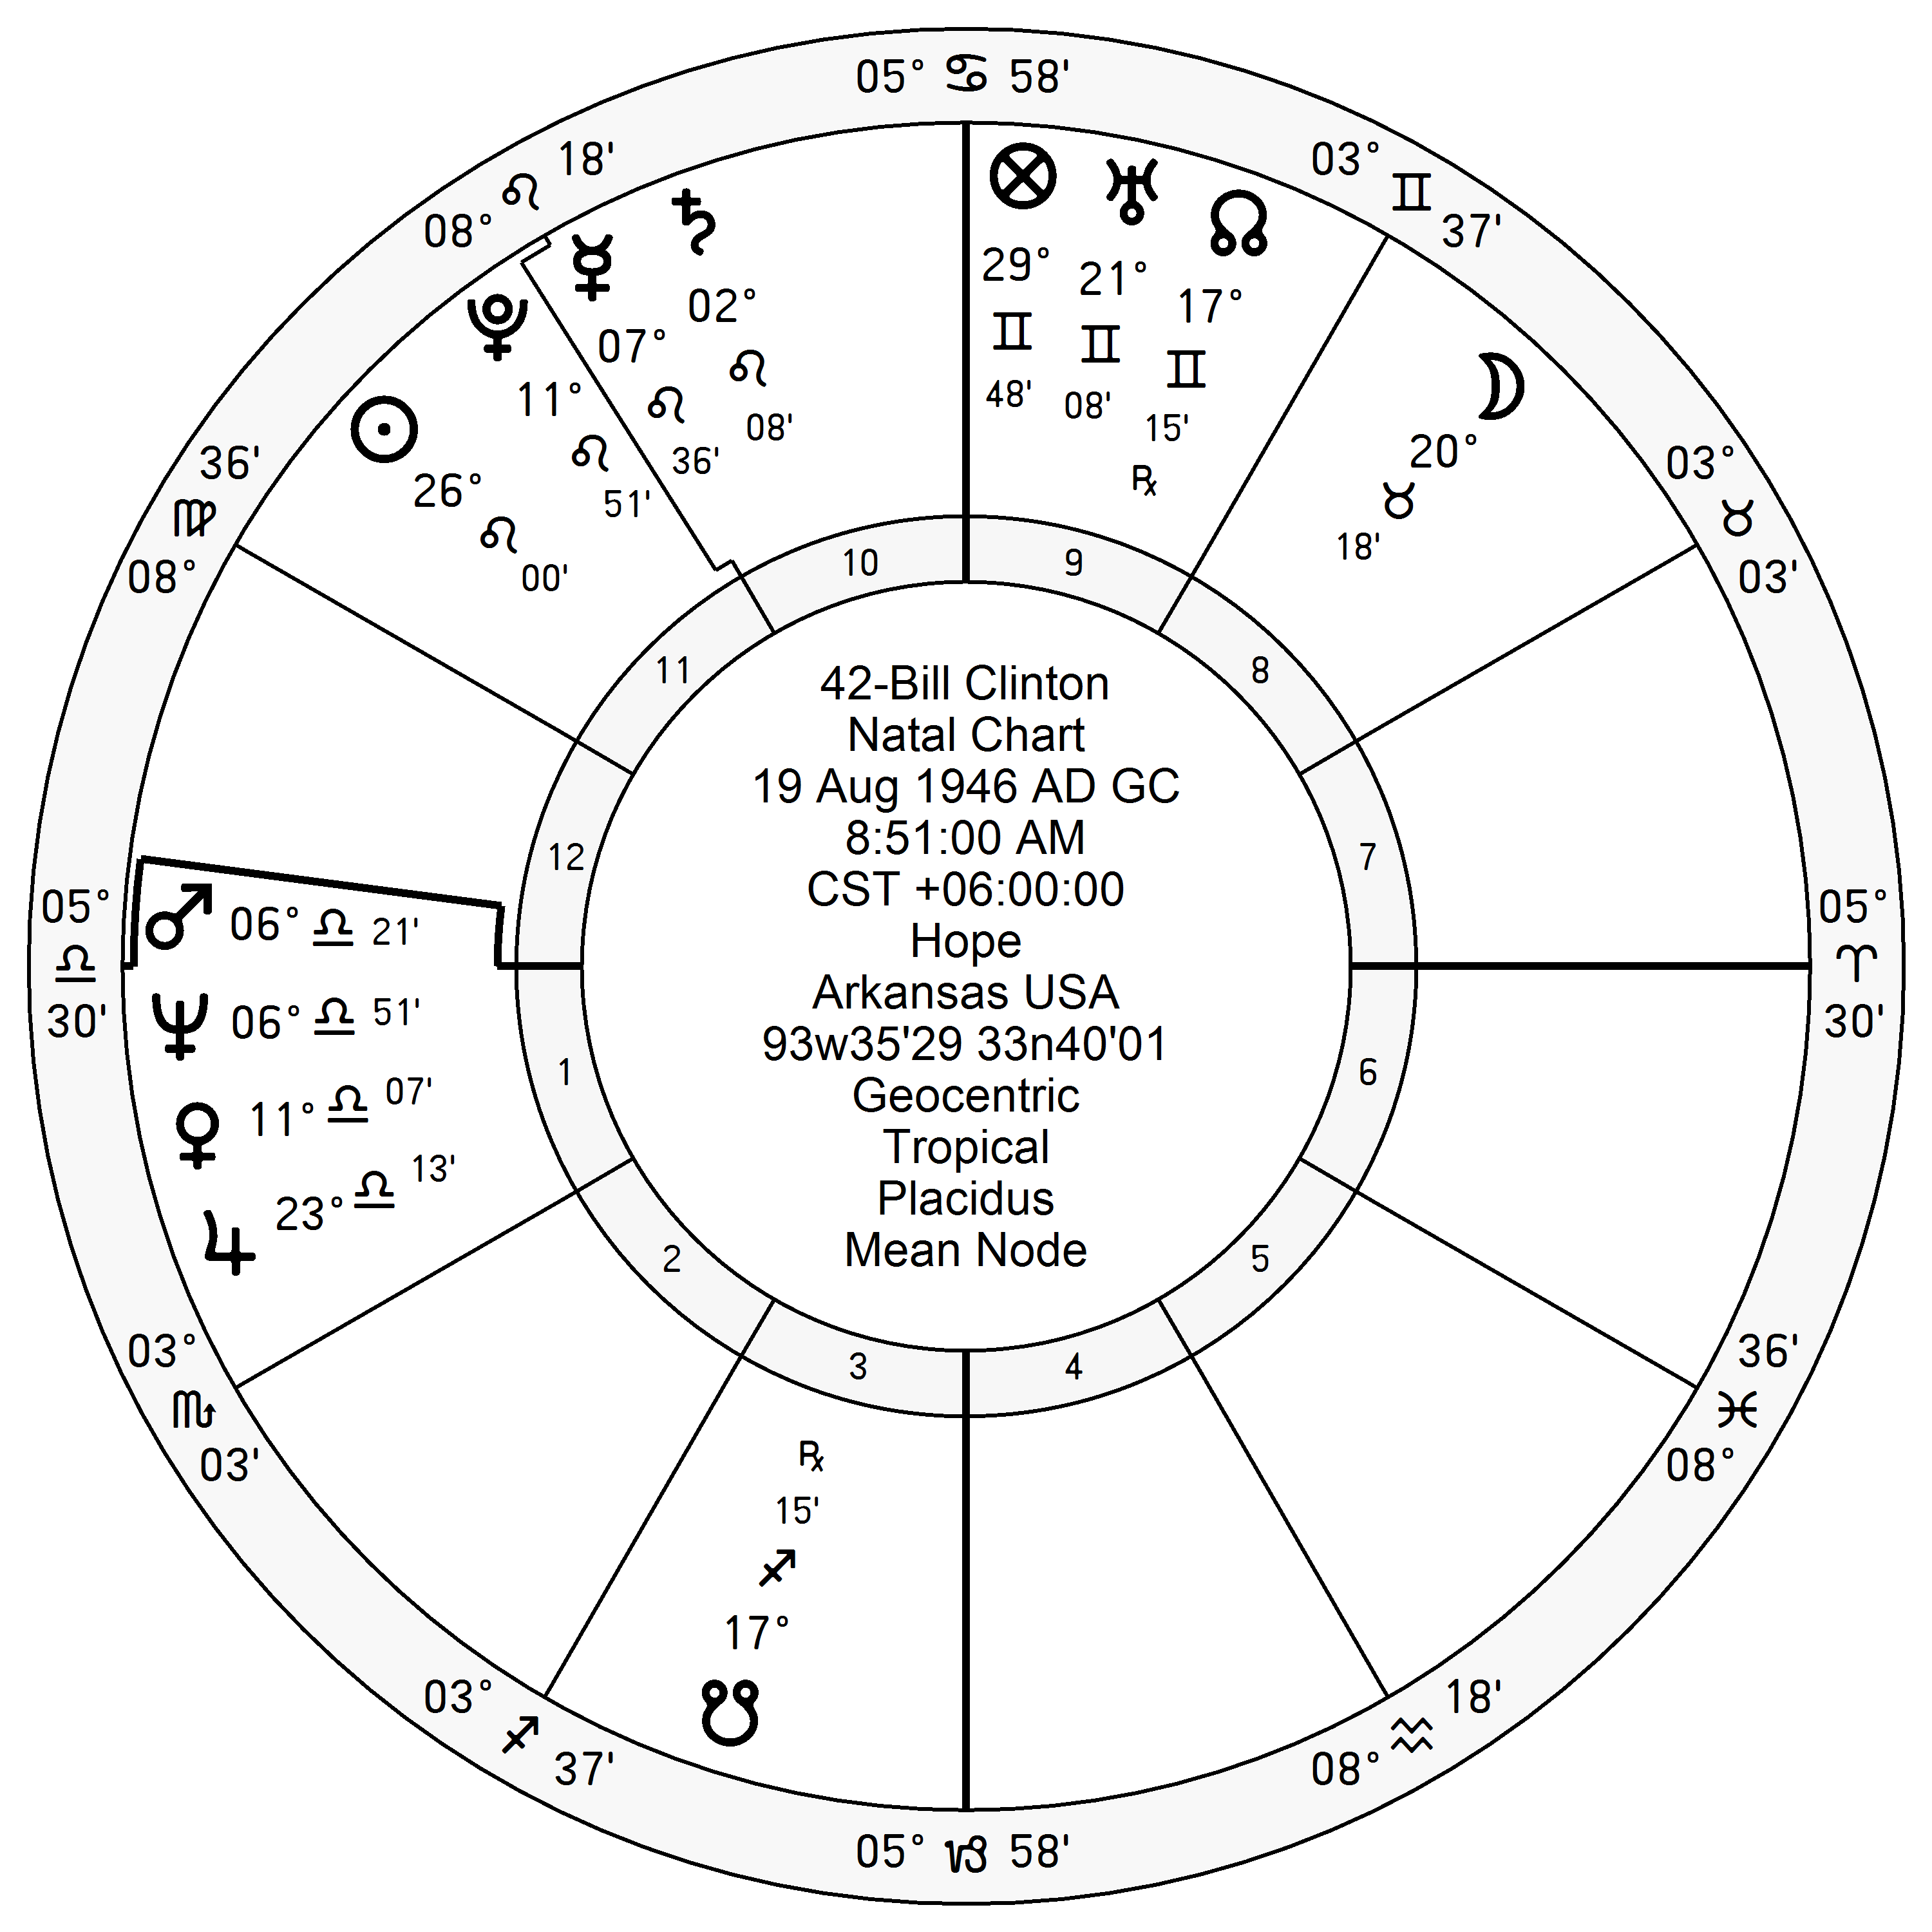
\includegraphics[width=0.9\textwidth]{charts/Clinton.png}}
\fontsize{8pt}{9pt}\selectfont

\Sun\, in \Leo\, in P1 \Square\, P10; \Sextile\, N1 \\
\Venus\, \Sextile\, P1; in \Libra\, in N1 \Square\, N10

\column{0.48\textwidth}
\vspace{-1em}
{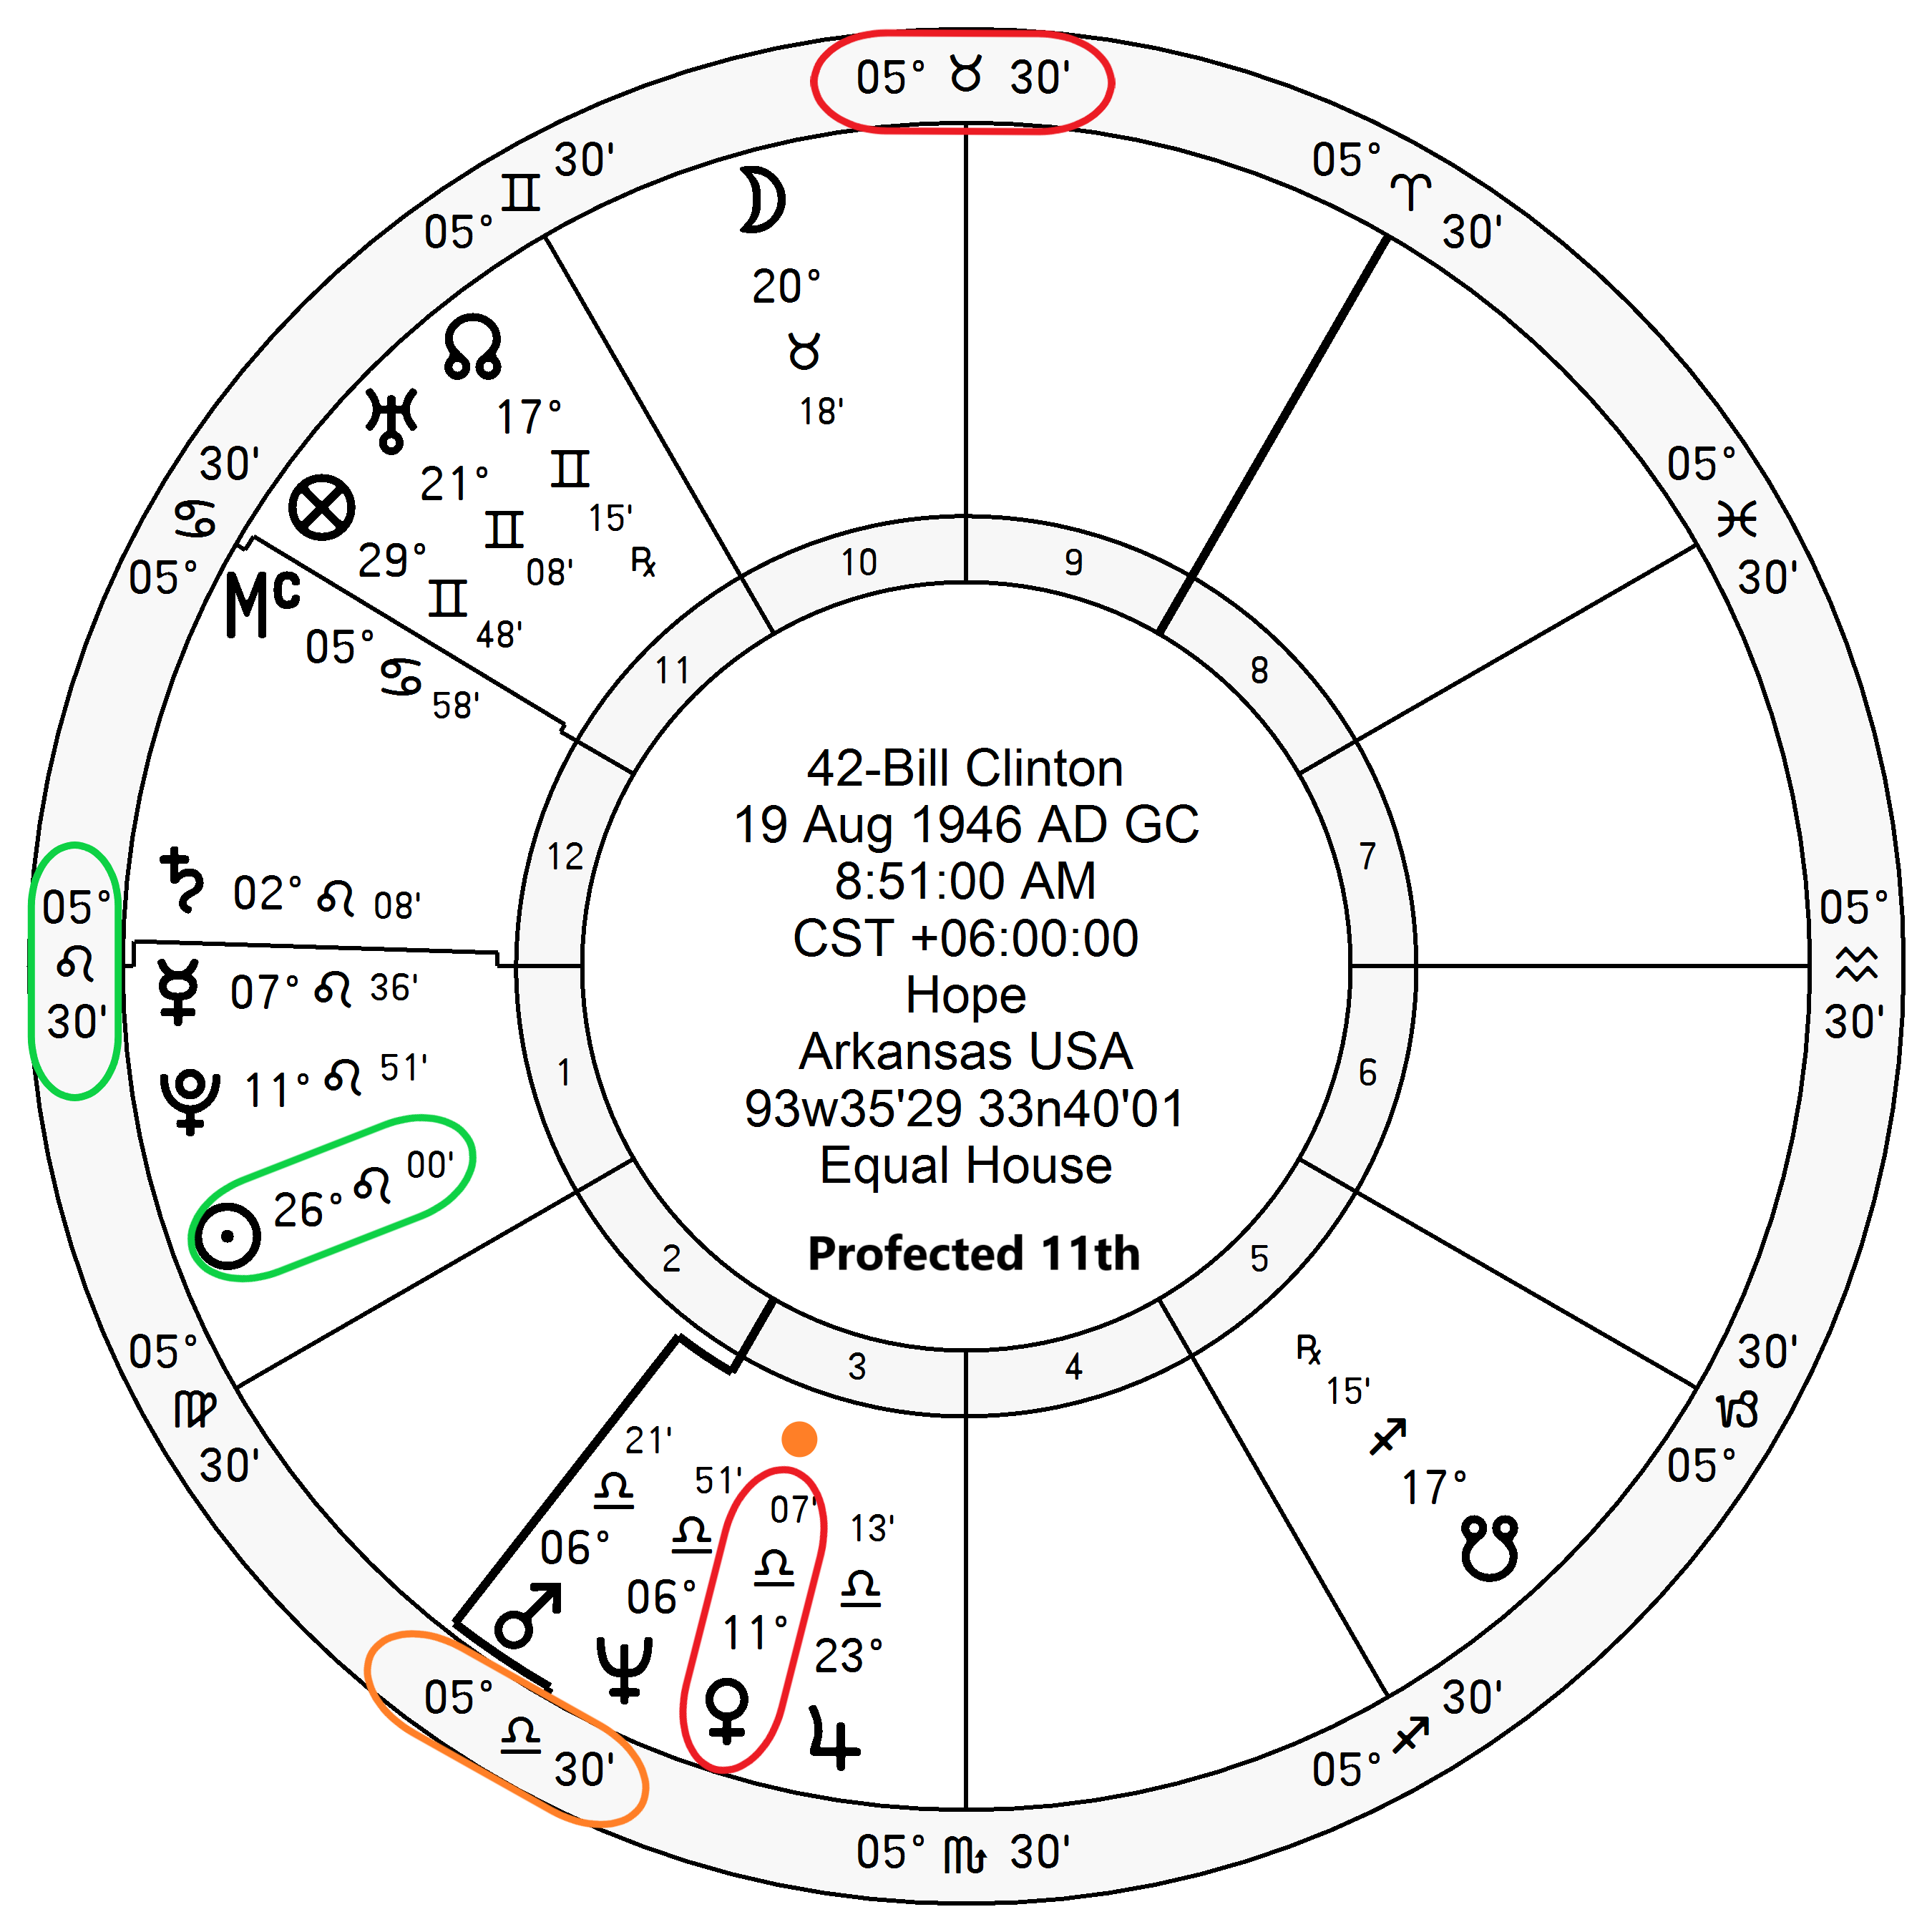
\includegraphics[width=0.9\textwidth]{charts/Clinton-Prof-11th.png}}
\fontsize{8pt}{9pt}\selectfont

\textbf{\dgreen P1=N11}
	$\Rightarrow$ \Sun\, $\Rightarrow$ \textbf{\dgreen P1/N11}\\
\textbf{\red P10}=N8
	$\Rightarrow$ \Venus\, $\Rightarrow$ \textbf{\red P3}/\textbf{\dgreen N1}\\
PE=\textbf{\red P3}\textbf{\dgreen /N1}
	 $\Rightarrow$ \Venus\, $\Rightarrow$ \textbf{\red P3}/\textbf{\dgreen N1}

\end{columns}
\end{frame}

% ===================================================
\begin{frame}[t]{Election November 3, 1992: George H.W. Bush}
\small
\begin{columns}[T, onlytextwidth]
\column{0.48\textwidth}
\vspace{-1em}
{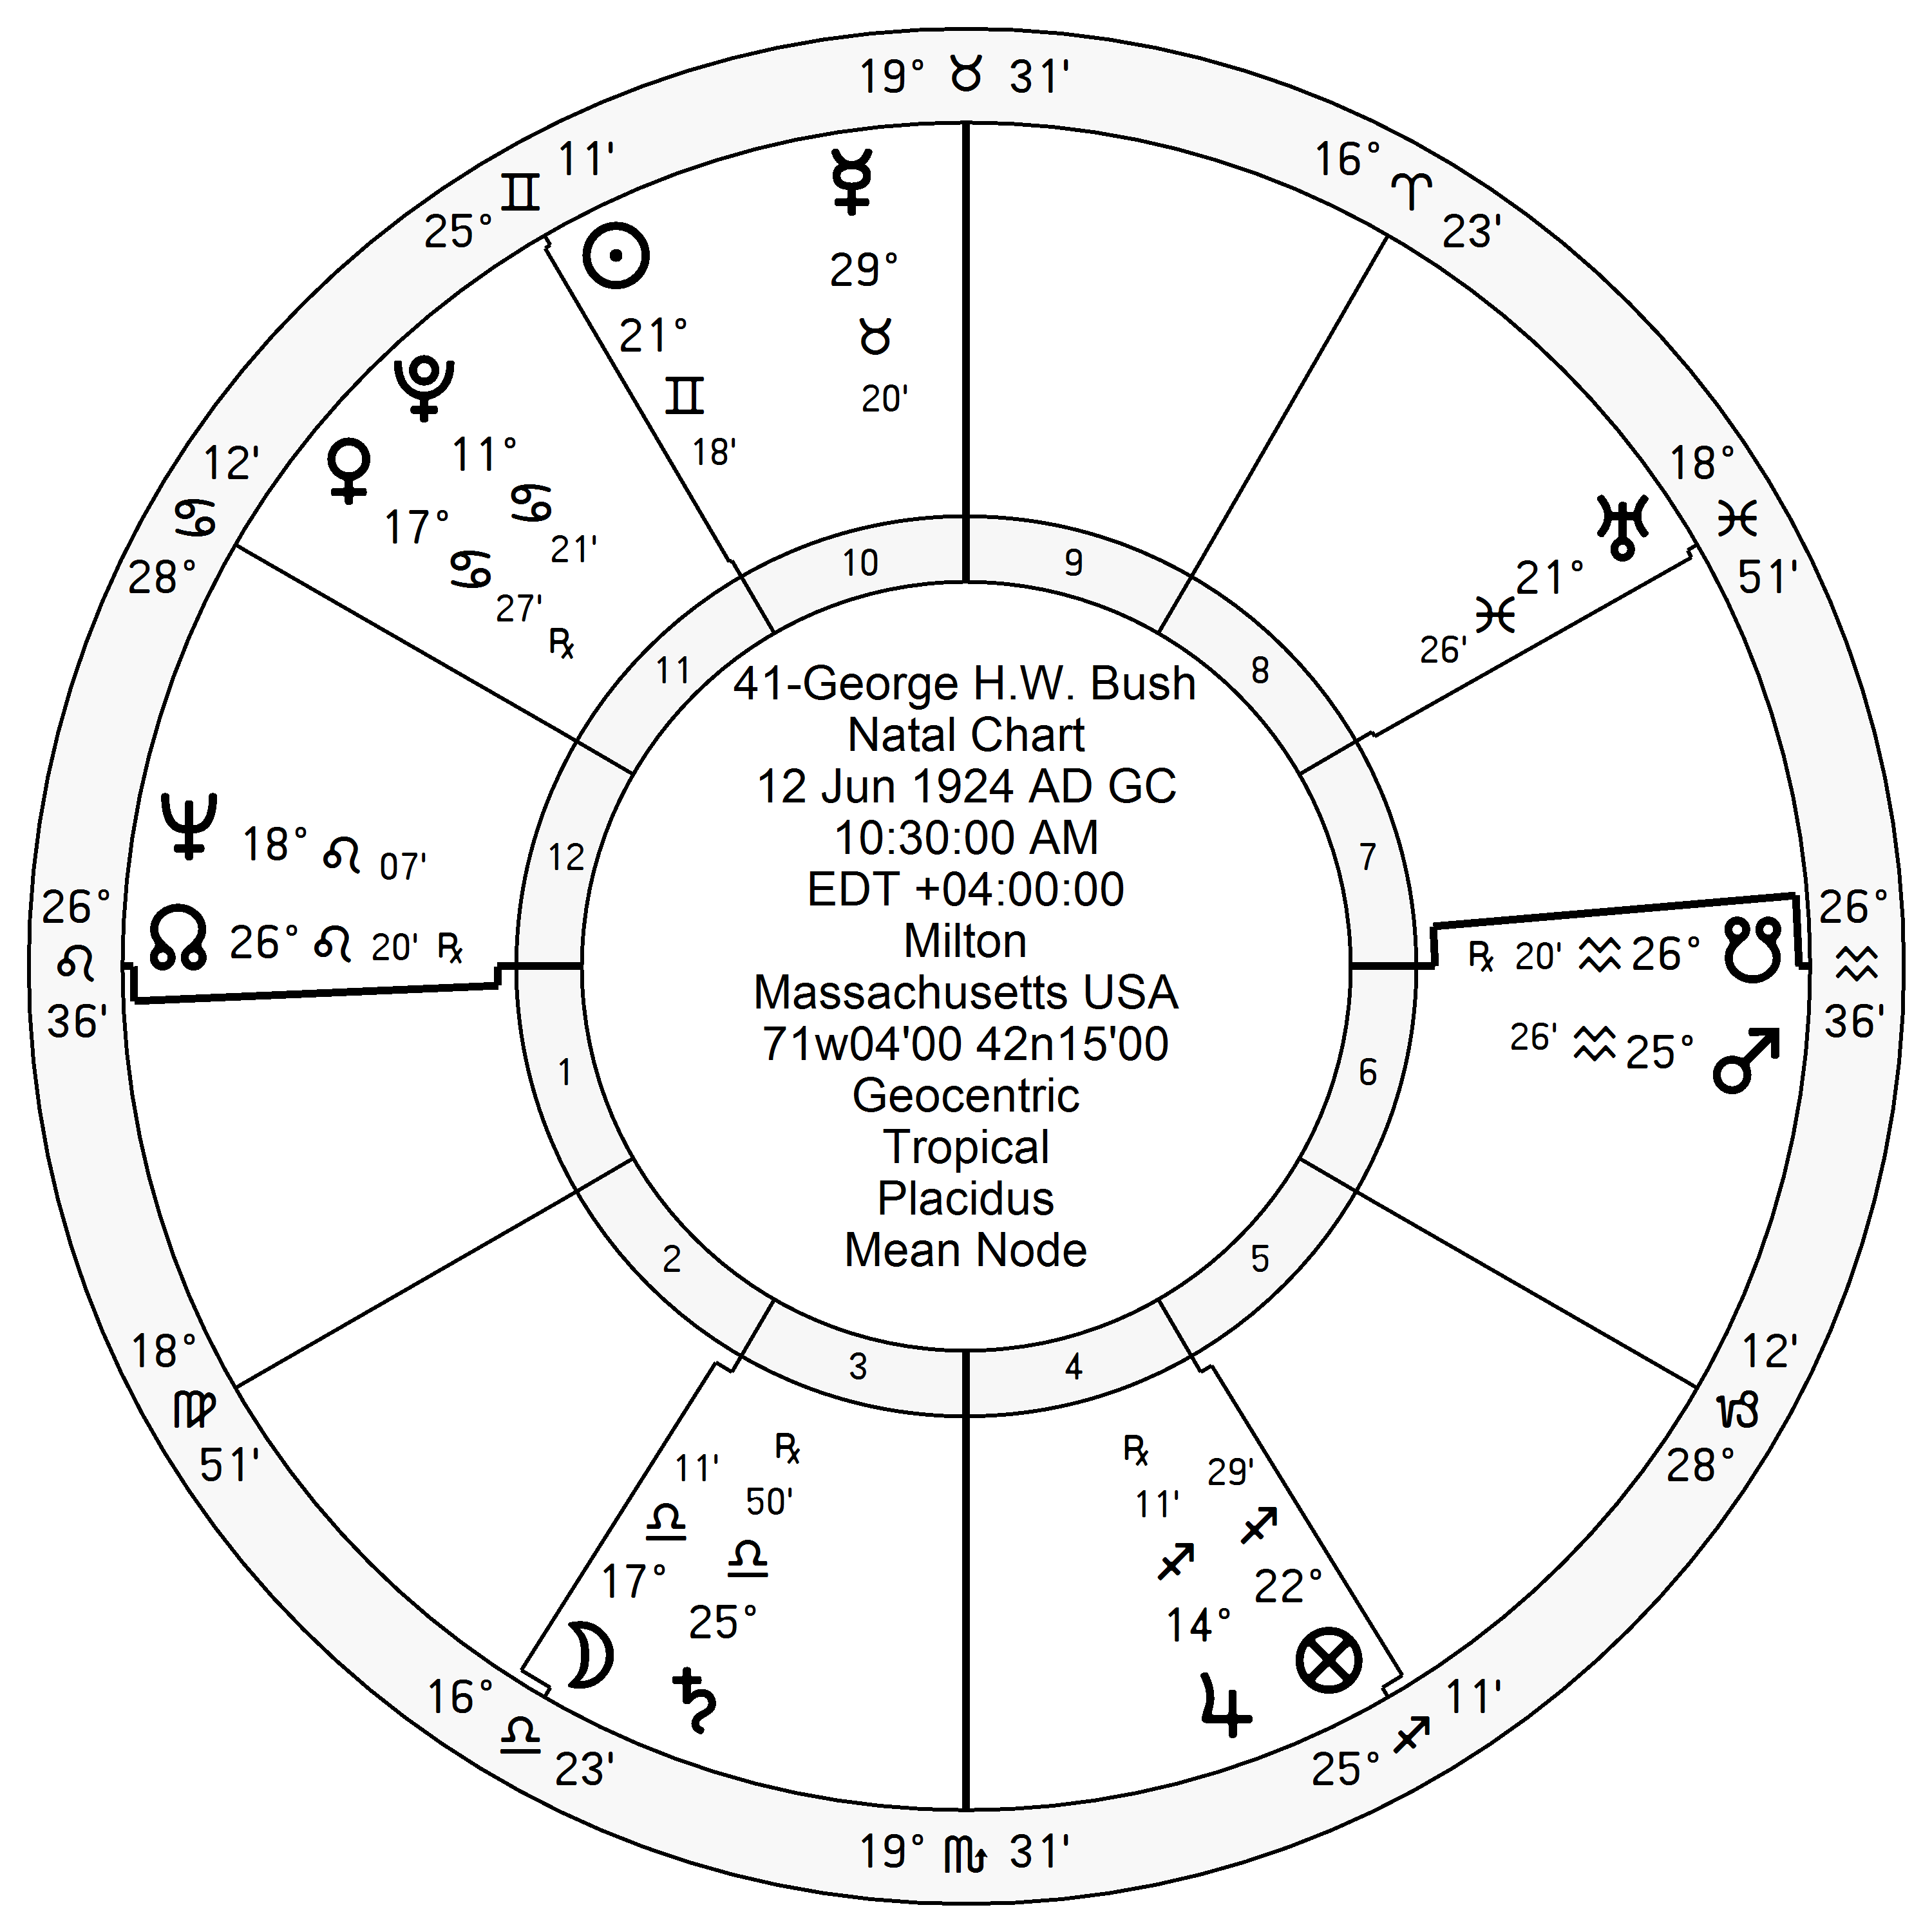
\includegraphics[width=0.9\textwidth]{charts/GHW-Bush.png}}
\fontsize{8pt}{9pt}\selectfont

\Mars\, \Conjunction\, \SouthNode\, in P10; \Square\, N10 \\
\Saturn\, partile \Trine\, \Mars\, in P10; mitigated \Quincunx\, (\Opposition) N10 \\
\Sun\, \Trine\, P10; in N10, \Square\, N1 \\
\vspace{0.5em}
Another case of the \SouthNode\, weakening the candidate's chances?

\column{0.48\textwidth}
\vspace{-1em}
{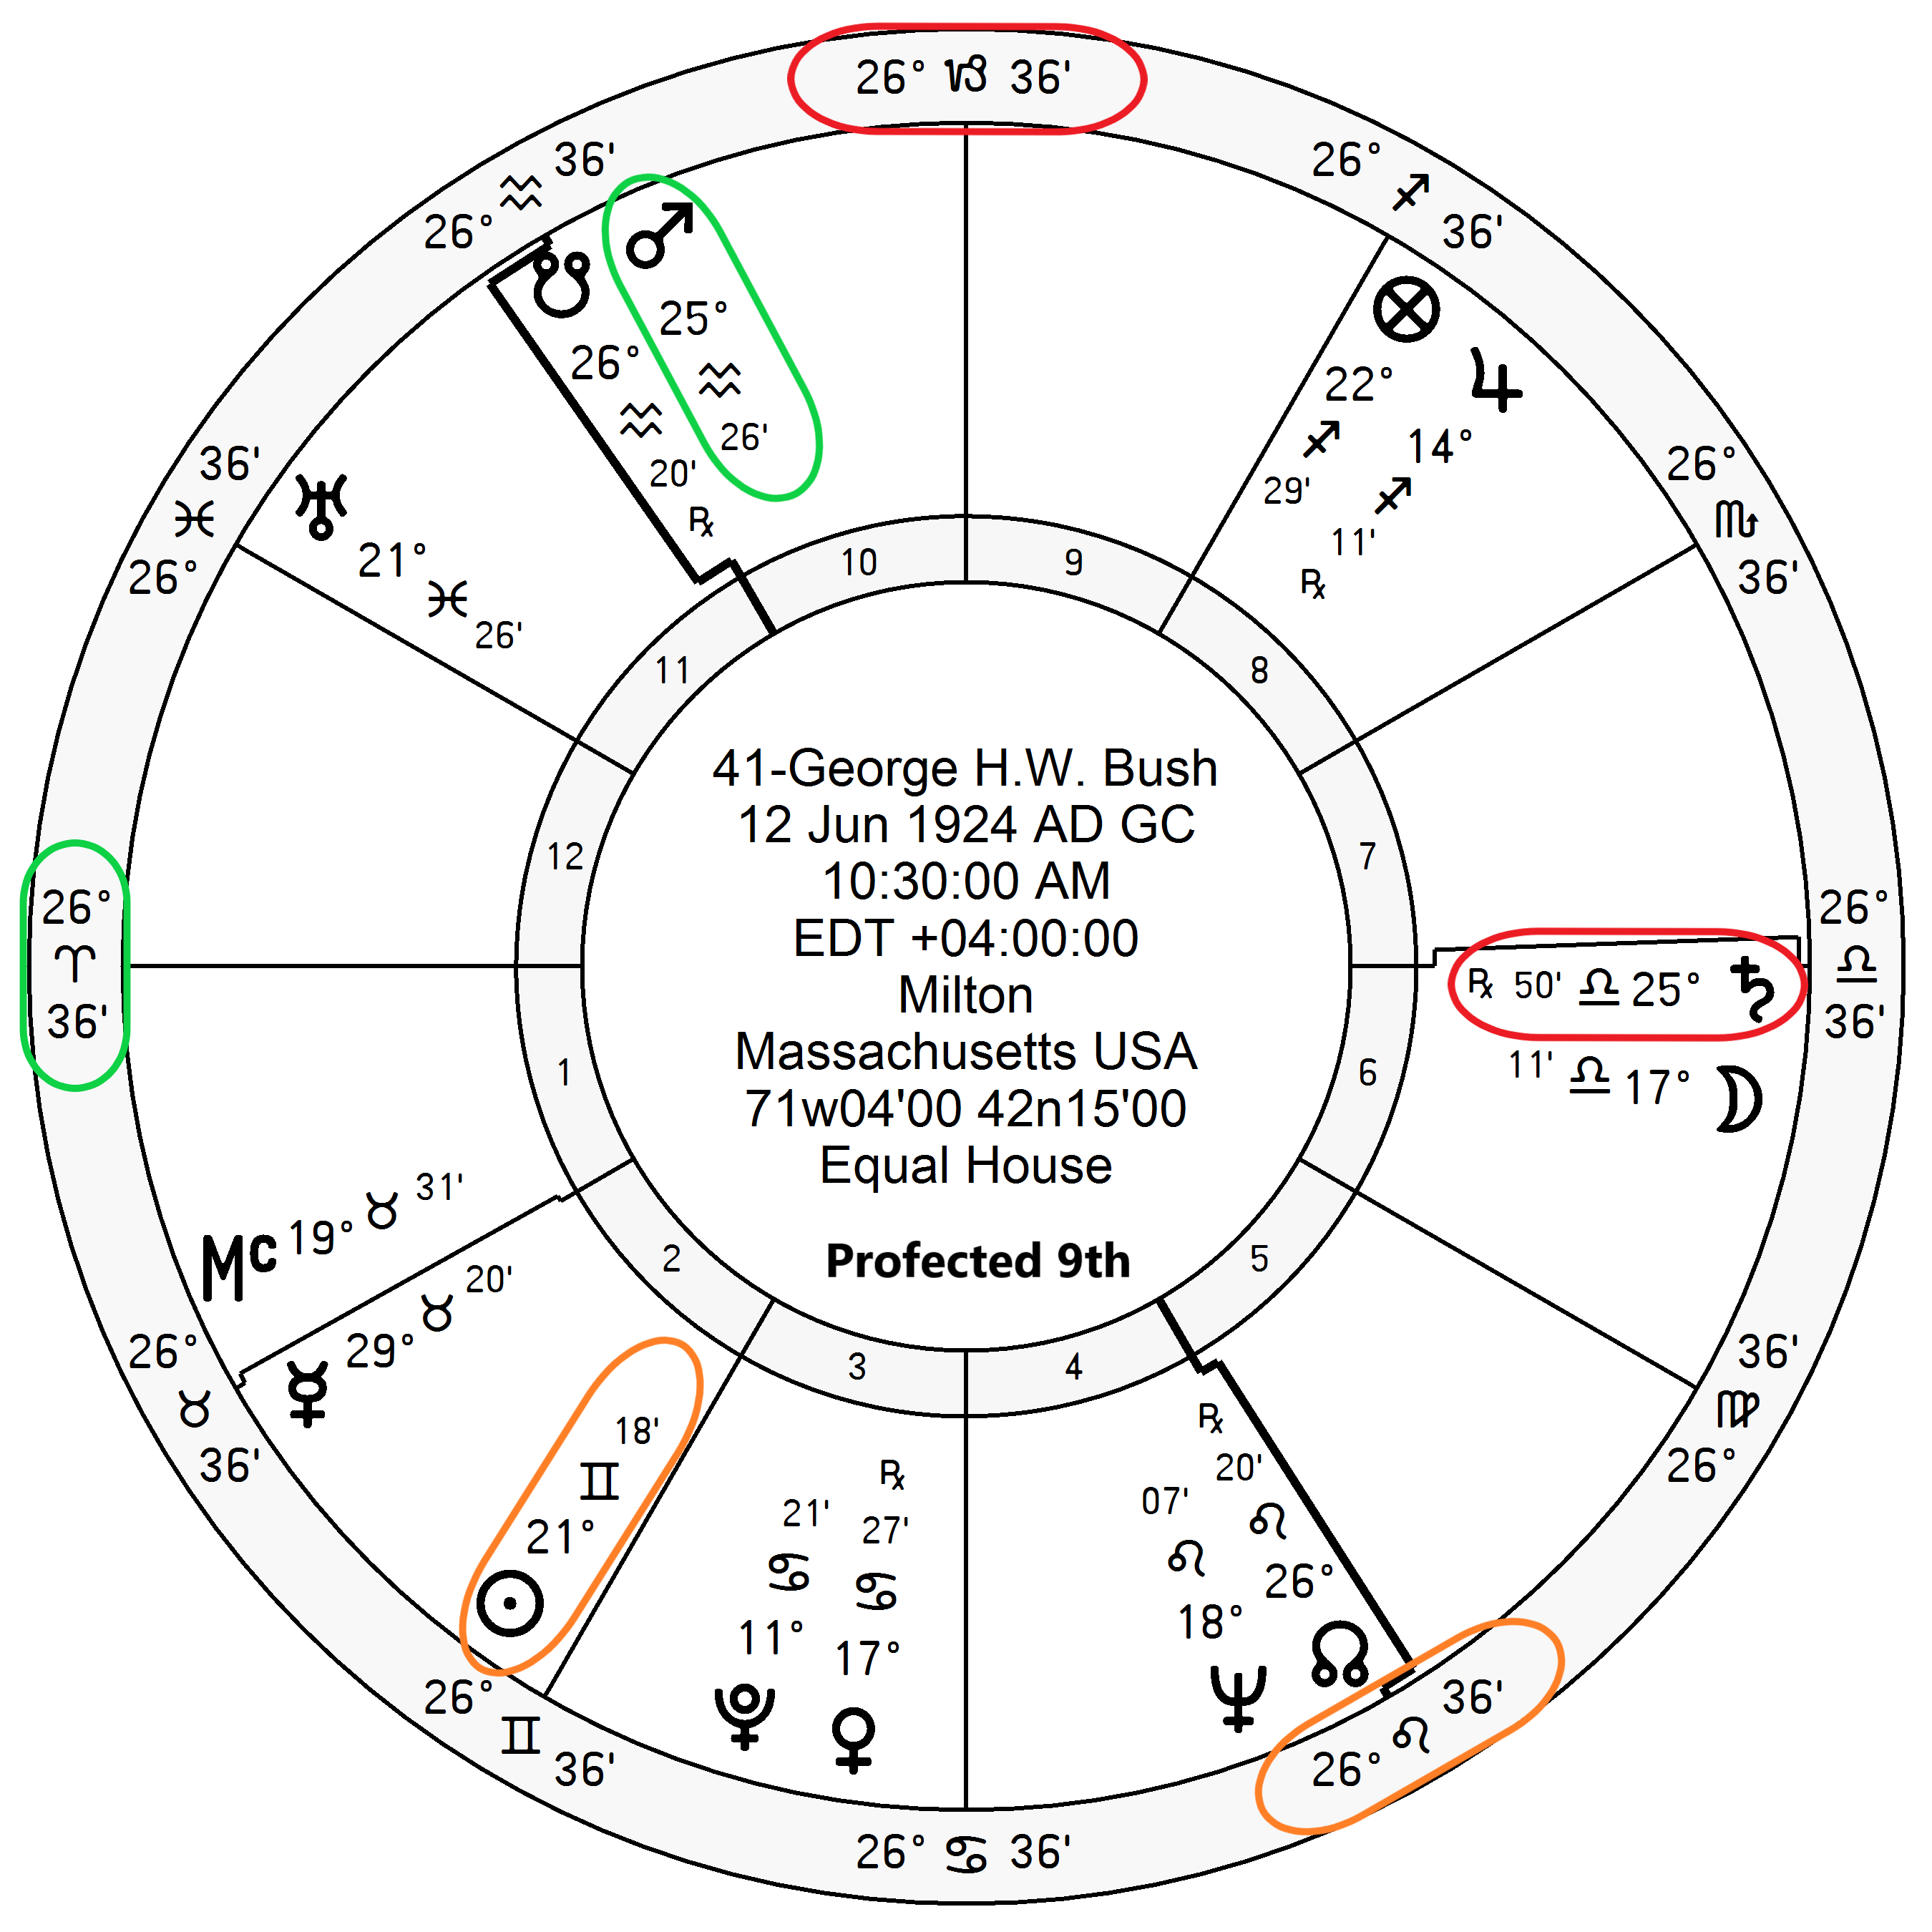
\includegraphics[width=0.9\textwidth]{charts/GHW-Bush-Prof-9th.png}}
\fontsize{8pt}{9pt}\selectfont
\textbf{\dgreen P1}=N9
	$\Rightarrow$ \Mars\, (\Conjunction\, \SouthNode) 
	$\Rightarrow$ \textbf{\red P10/N6}\\
\textbf{\red P10=N6}
	$\Rightarrow$ \Saturn\, (partile \Trine\, \Mars) $\Rightarrow$ \textbf{\red P6}/N3\\
PE=P5/\textbf{\dgreen N1}
	 $\Rightarrow$ \Sun\, $\Rightarrow$P2/\textbf{\red N10}

\end{columns}
\end{frame}
